\documentclass[a4paper,12pt]{report}

\usepackage{alltt, fancyvrb, url}
\usepackage{graphicx}
\usepackage[utf8]{inputenc}
\usepackage{float}
\usepackage{hyperref}

% Questo commentalo se vuoi scrivere in inglese.
\usepackage[italian]{babel}

\usepackage[italian]{cleveref}

\title{Relazione \\``Time2Survive''}

\author{Andrea Cecchini \\ Nicolò D'Addabbo \\ Luca Oskari Fiumanò \\Leonardo David Matteo Magnani}
\date{\today}


\begin{document}

\maketitle

\tableofcontents

\chapter{Analisi}

\section{Requisiti}
Il progetto si pone l’obiettivo di creare un videogioco survival shoot ‘em up ispirato a ``The Binding of Isaac'' \footnote{\url{https://store.steampowered.com/app/113200/The_Binding_of_Isaac/}}.
Con survival shoot ‘em up si intende un genere di videogioco nella quale l’obiettivo è sopravvivere il più a lungo possibile a ondate di nemici, generandone di nuove una volta eliminata la precedente.

\subsection*{Requisiti funzionali}
\subsubsection{Requisiti Funzionali Obbligatori}
\begin{itemize}
	\item Il gioco dovrà occuparsi di gestire la partita dell’utente all’interno della mappa di gioco di Time2Survive, rendendo più difficile la sopravvivenza del giocatore attraverso ondate di nemici di difficoltà crescente.
    All’interno della mappa, il giocatore potrà:
    \begin{itemize}
        \item Sfruttare le proprie abilita’ di videogiocatore per sopravvivere alle numerose ondate dei nemici che si susseguiranno.
        \item Sfidare ondate che verranno generate al completamento della precedente. Le ondate terminano quando tutti i nemici sono stati eliminati.
        \item I nemici si potranno eliminare attraverso l'utilizzo di proiettili generati dal personaggio.
        \item La partita sarà conclusa alla morte virtuale del giocatore.
    \end{itemize}
	\item Il giocatore si troverà all'interno di una stanza in cui verranno generate le ondate di nemici.
	\item La difficoltà del gioco sarà incrementale e riguarderà sopratutto le ondate. Essa sarà manipolata attraverso 3 parametri:
    \begin{itemize}
        \item Numero: numero dei nemici a schermo.
        \item Resilienza: resistenza agli attacchi da parte del giocatore.
        \item Forza: danno provocato dal nemico.
    \end{itemize}
	\item Il giocatore si potrà muovere nell’ambiente di gioco costituito da una singola stanza.
    \item I nemici sono delle entità attive del gioco che cercano di eliminare il giocatore.
    Vengono controllati da una semplice AI (Artificial Intelligence). 
	Per intelligenza artificiale si intende un software che conferisce a ogni nemico una strategia di movimento e di combattimento.
    \item Il giocatore dovrà essere in grado di capire lo stato della partita in ogni momento della suddetta visualizzando la propria vita. 
	Il giocatore sarà inoltre in grado di visualizzare le proprie capacità essendo in grado di visualizzare il numero di ondate alle quali è sopravvissuto.
\end{itemize}

\subsubsection{Requisiti Funzionali Opzionali}
\begin{itemize}
	\item Per aiutare il giocatore, saranno disponibili diversi potenziamenti che gli permetteranno di aumentare le proprie abilità.
	\item Per rendere più vario la partita saranno presenti diversi tipi di nemici con caratteristiche uniche e diverse tra loro.
\end{itemize}
\subsection*{Requisiti non funzionali}
\begin{itemize}
	\item Il programma deve mantenere un profilo di prestazione adeguato e costante nonostante il variare dello stato del mondo di gioco alla fine di garantire un’esperienza di gioco fluida e gradevole.
	\item Per rendere il videogioco il più godibile possibile la grafica dovrà essere elaborata con uno stile grafico al passo coi tempi.
\end{itemize}
\newpage
\section{Analisi e modello del dominio}
T2S mette a disposizione del giocatore la possibilità di giocare una nuova partita.
\\
Una partita gestisce il proprio stato e il mondo di gioco di T2S.
\\
Il mondo di T2S è l’arena dove le diverse entità interagiscono fra di loro.
\\
Al giocatore sarà data la possibilità di controllare una di queste entità, il quale sarà l’avatar del giocatore nella partita.
\\
Durante lo svolgimento della partita verranno generate delle ondate di entità controllate da un’intelligenza artificiale con il compito di attaccare e uccidere l’avatar del giocatore.
\\
Per combattere questi nemici, l’avatar avrà la possibilità di sparare dei proiettili che possono essere migliorati tramite potenziamenti.
\\
Una volta sconfitta un’ondata viene aggiornato lo stato della partita incrementando il numero di round alla quale si è sopravvissuti e viene generata una nuova ondata di maggiore difficoltà.
\\
All’inizio della partita all’avatar verranno assegnati dei proiettili di default e un determinato numero di punti vita.
\\
Una volta subito un danno, a seconda della sua entità, verrà detratta una certa quantità dalla vita corrente.
\\
La partita termina quando il giocatore ha perso tutti i suoi punti vita.
\\
Le difficoltà che il progetto si porta dietro sono:
\begin{itemize}
	\item Un’implementazione di un intelligenza artificiale in grado di controllare correttamente i nemici. La prima versione del gioco fornirà ai nemici un Controller basato sulle coordinate del player nella mappa. 
	\item Una grafica completa che verrà implementata inizialmente in maniera minimale.

\end{itemize}

\begin{figure}[H]
\centering{}
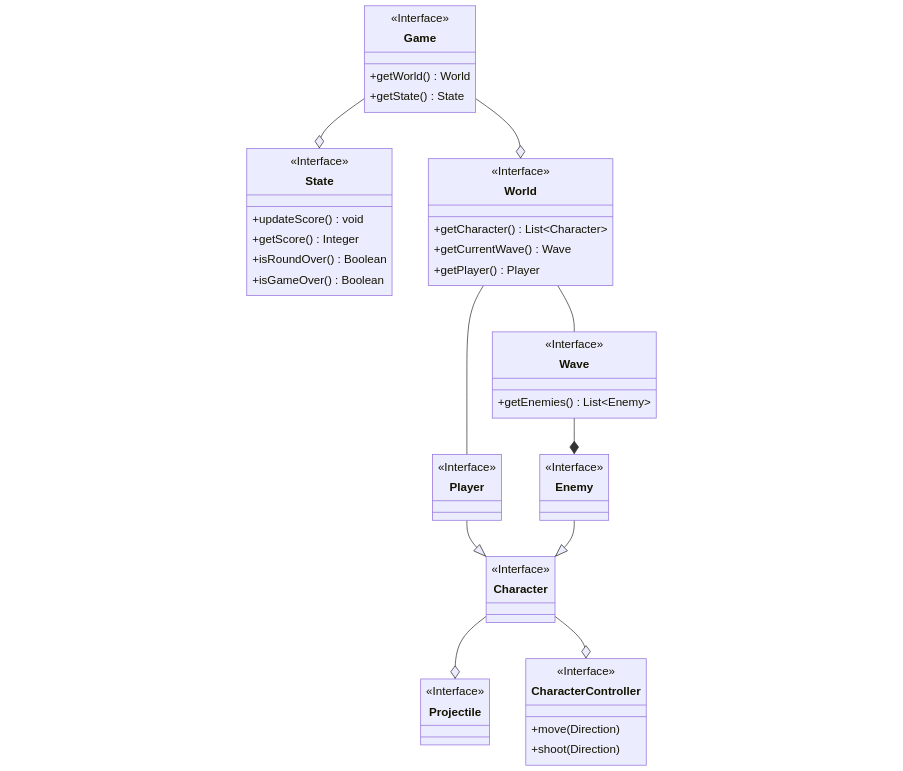
\includegraphics[width=1\textwidth]{img/Schema-UML-Analisi.png}
\caption{Schema UML dell'analisi del problema, con rappresentate le entità principali ed i rapporti fra loro}
\label{img:analysis}
\end{figure}




\chapter{Design}
\section{Architettura}
T2S è stato sviluppato adottando un pattern architetturale che mantenesse una simile struttura MVC, quindi con i suoi vantaggi, contaminandola però attraverso l’utilizzo del pattern Component.
\\
Il pattern Component permette ad una singola entità di estendersi su domini multipli senza accorparli in unica classe.
\\
Applicandolo al dominio dell’applicazione (Model), avremo che ogni entità risulta essere un GameObject.
\\
Tale GameObject viene adornato con dei GameComponent, ognuno dei quali appartiene ad un dominio (Input,Fisica,Stato,Grafica …) particolare.
\\
Ogni GameComponent è responsabile per l’aggiornamento del GameObject nel rispettivo dominio.
\\
Tuttavia, pur appartenendo a domini diversi, i diversi GameComponents potrebbero aver bisogno di comunicare tra di loro.
\\
Sfruttando come “container” il GameObject stesso è stato messo a disposizione dei GameComponents un semplice ma funzionale sistema di messaggistica.
\\
L’utilizzo di questi componenti porta ad importanti vantaggi:
\begin{itemize}
	\item \textbf{Stroncamento di un albero di ereditarietà troppo complesso e lungo}:
	Per rappresentare entità con diversi comportamenti si utilizza la composizione di GameComponent che implementino quei comportamenti, senza nessun utilizzo dell’ereditarietà.
	%
	\item Eliminazione del problema \textbf{Deadly Diamond of Death}
	%
	\item \textbf{Riduzione al minimo delle ripetizioni di codice} dovuto alla creazione di componenti altamente riutilizzabili
\end{itemize}
Dal punto di vista del pattern architetturale Model-View-Controller, i rispettivi moduli sono rappresentati da:
\begin{itemize}
	\item \textbf{Model}:
	Viene seguito il seguente mantra “Everything is a GameObject”		
Difatti ogni entità del dominio viene rappresentata e astratta grazie all’utilizzo 	dell’interfaccia GameObject, la quale svolge il ruolo di “container” di GameComponents.
	%
	\item \textbf{Controller}:
 Questo ruolo viene affidato all’interfaccia GameEngine, la quale ha il compito di gestire l’aggiornamento di ogni GameObject e dei suoi componenti e la renderizzazione sulla View.
	%
	\item \textbf{View}:
 Il ruolo della view viene demandato a due interfacce ben connesse tra di loro: Scene  e Graphics.
L’interfaccia Scene astrae il concetto di “Scena” di gioco
L’interfaccia Graphics ha il compito di saper “disegnare” i diversi GameObjects con la 
tecnologia grafica dipesa dall’implementazione e fornita dall'implementazione di Scene.
\end{itemize}
Dal diagramma delle classi, qui sotto fornito, è possibile notare un elemento di differenza rispetto ad una classica architettura MVC: un componente di spicco,denominato GraphicsComponent, risulta avere dei riferimenti alla parte di view e di model, creando un collegamento che a prima vista potrebbe risultare problematico.
%
La modularità di M.V.C. non viene però attaccata: volendo, come esempio, cambiare la tecnologia di sviluppo per quanto riguarda la grafica si modificherà esclusivamente la parte di View dell'applicazione, senza ripercussioni in nessun altro modulo del programma.
%
L’ipotetico passaggio da JavaFx e Swing, dunque, non risulta essere problematico: 
%
si dovranno sostituire le implementazioni di JavaFx delle interfacce Graphics e Scene con delle nuove implementazioni che utilizzino Swing.

\begin{figure}[H]
\centering{}
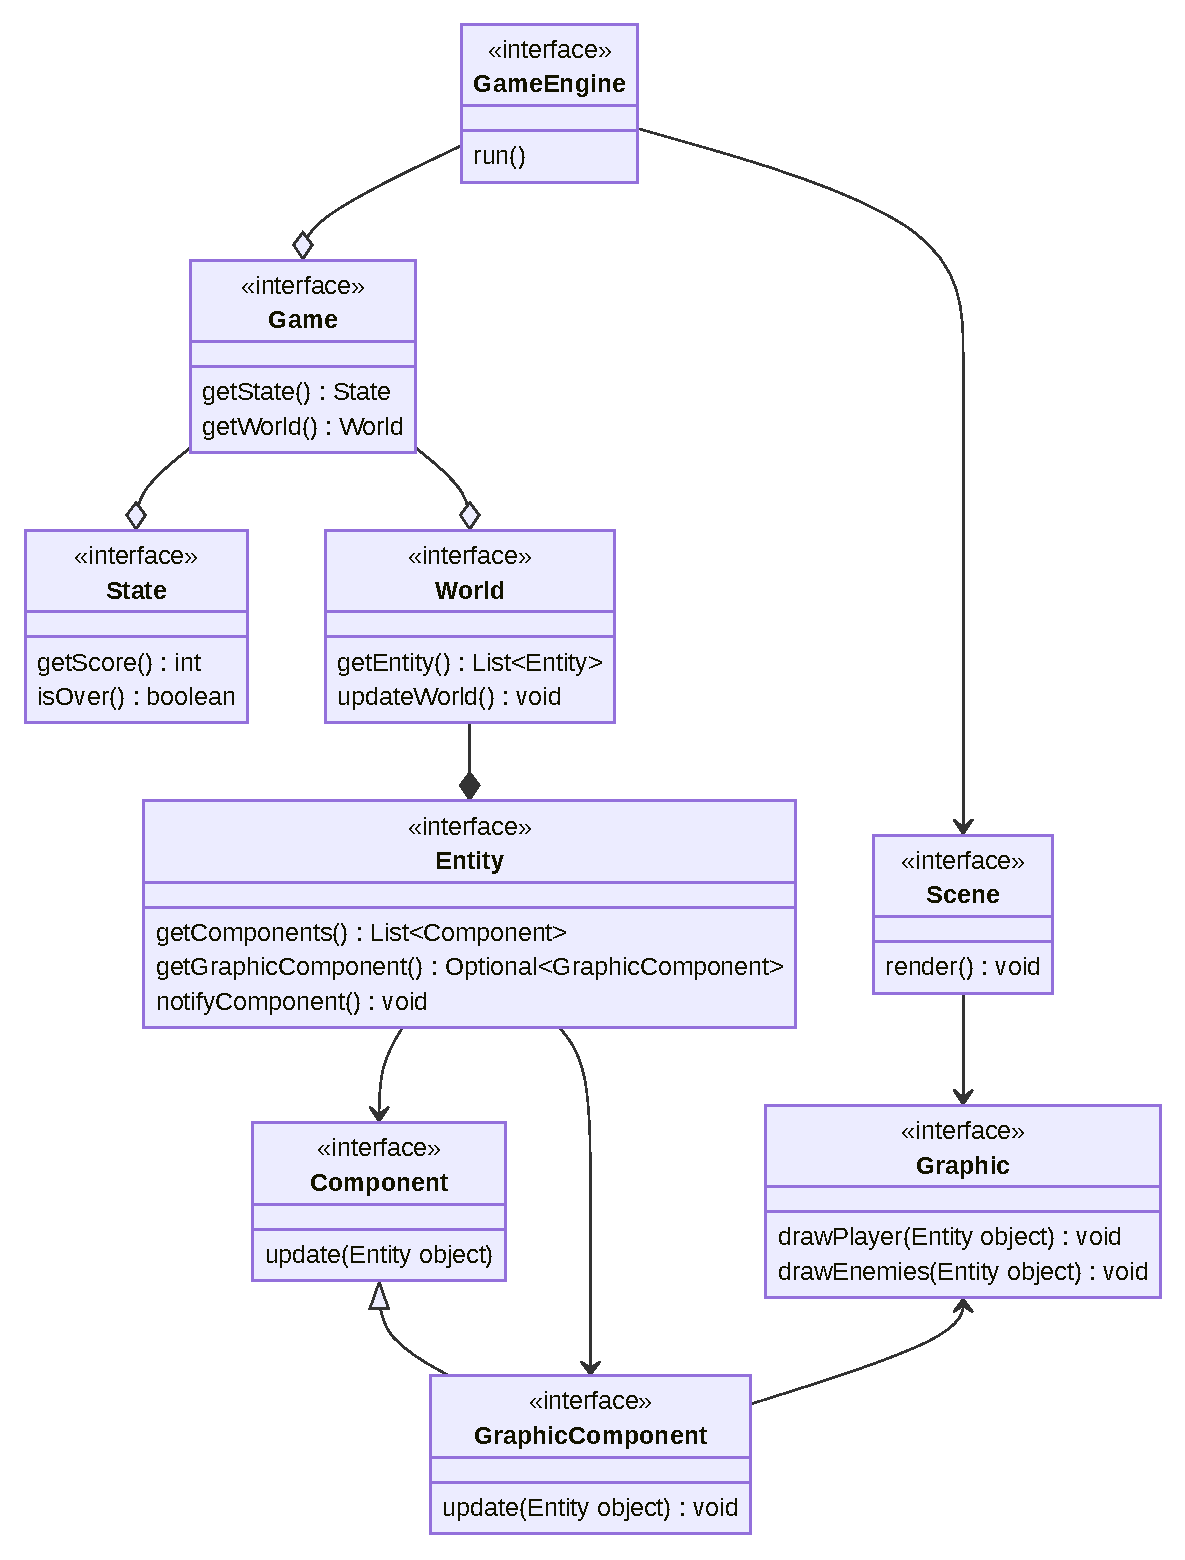
\includegraphics[width=1\textwidth]{img/SoftwareArchitectureUML.pdf}
\caption{Schema UML architetturale di T2S.}
\label{img:analysis}
\end{figure}

\section{Design dettagliato}

\subsection*{Nicolò D'Addabbo}

\subsubsection{Input Controller intercambiabili}

\begin{figure}[H]
\centering{}
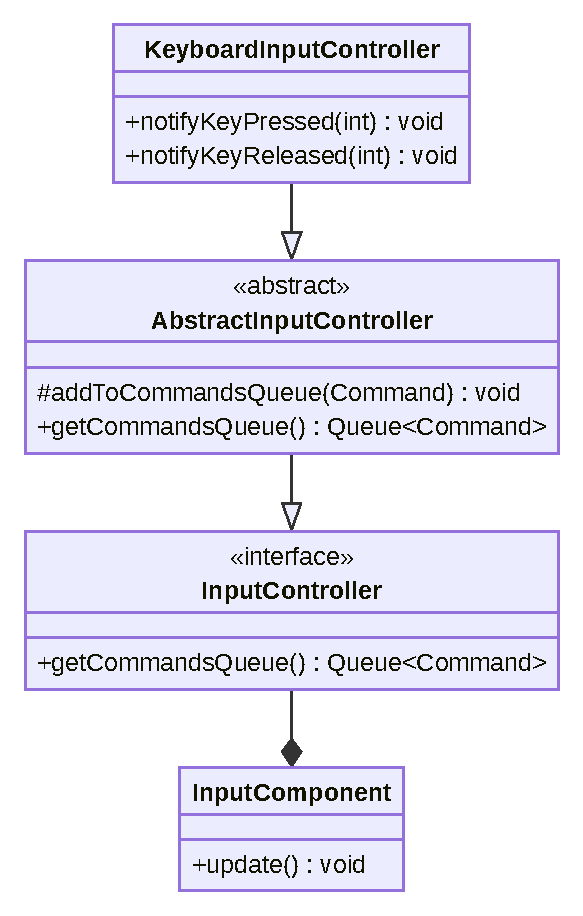
\includegraphics[scale=0.75]{img/InputControllerUML}
\caption{Rappresentazione UML del pattern Strategy per l'Input Component}
\label{img:strategy}
\end{figure}

\paragraph{Problema} Un’entità può ricevere input da diverse sorgenti come ad esempio una tastiera o un joypad, 
la cui presenza non è di interesse dell’entità stessa. 
Infatti deve possedere solo un generico Input Component con un metodo update.

\paragraph{Soluzione} La classe \textbf{InputComponent} implementa lo \textit{Strategy pattern}, contenendo un riferimento a un \textit{InputController} che funge da strategia per la gestione dell'input. Quest'ultimo può essere sostituito con un'implementazione diversa, permettendo l'utilizzo di strategie differenti.
\\
Il metodo \textit{update} dell’Input Component chiama il metodo \textit{execute} su ogni \textit{Command} (come descritto nella sezione "Gestione dei comandi di gioco") presente nella coda di comandi restituita dall'\textit{InputController} (come descritto nella sezione "Input Controller con molteplici stati").
\\
Inoltre, grazie allo \textit{Strategy pattern}, è possibile sviluppare un'intelligenza artificiale in modo semplice. Un'AI, infatti, non è altro che un \textit{InputController} che genera diversi \textit{Command} in base a un determinato algoritmo.
\\

\subsubsection{Gestione dei comandi di gioco}

\begin{figure}[H]
\centering{}
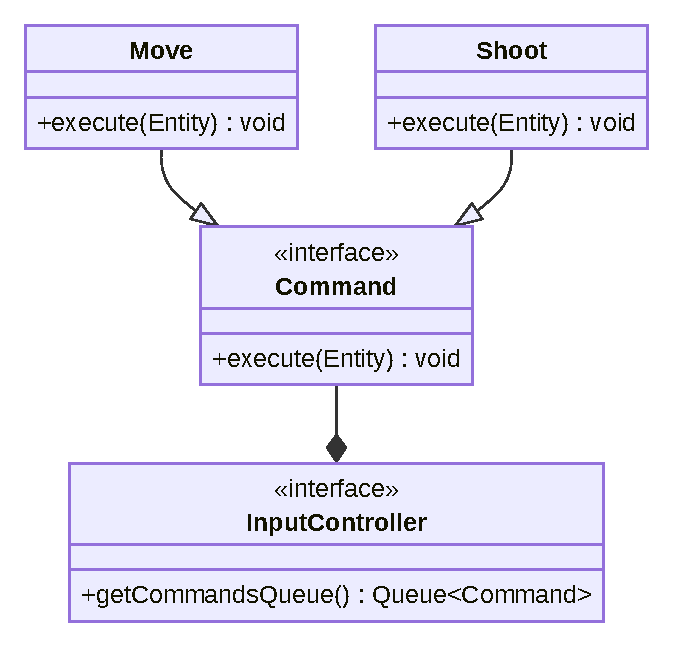
\includegraphics[scale=0.75]{img/CommandsUML}
\caption{Rappresentazione UML del pattern Command per la gestione dei comandi}
\label{img:command}
\end{figure}

\paragraph{Problema} Rendere riutilizzabili i comandi di gioco, separando la responsabilità di eseguirli dall’oggetto che li registra.

\paragraph{Soluzione} Il sistema di gestione dei comandi di gioco utilizza il \textit{Command pattern}. 
Questo pattern consente di incapsulare una richiesta, nel nostro caso un comando di input, in un oggetto. 
In questo modo il \textit{Command pattern} fornisce un livello di astrazione tra gli oggetti che triggerano azioni e quelli che le eseguono, 
riducendo la dipendenza tra questi oggetti.
La struttura del \textit{Command pattern} è composta da:
\begin{itemize}
\item \textbf{Command}: l'interfaccia che definisce l'operazione da eseguire. In questo caso rappresentato da \textit{Command}.
\item \textbf{Concrete Command}: classe che implementa l'interfaccia Command e specifica la logica di esecuzione per una determinata richiesta. In questo caso rappresentato da \textit{Move} e \textit{Shoot}.
\item \textbf{Receiver}: classe che contiene la logica vera e propria. I comandi gestiscono solo i dettagli di come una richiesta viene passata al \textit{receiver,} è infatti il \textit{receiver} che esegue il comando. In questo caso rappresentato dai diversi \textbf{Component}.
\item \textbf{Invoker}: classe che inizializza la richiesta. In questo caso rappresentato da \textbf{InputController + InputComponent}.
\end{itemize}
Altri vantaggi dell’utilizzo del \textit{Command pattern} sono la flessibilità e la riutilizzabilità. Infatti rende più facile l’aggiunta di nuovi comandi, la modifica di quelli esistenti o anche l’annullamento di comandi già eseguiti.

\subsubsection{Riuso di Input Controller}

\begin{figure}[H]
\centering{}
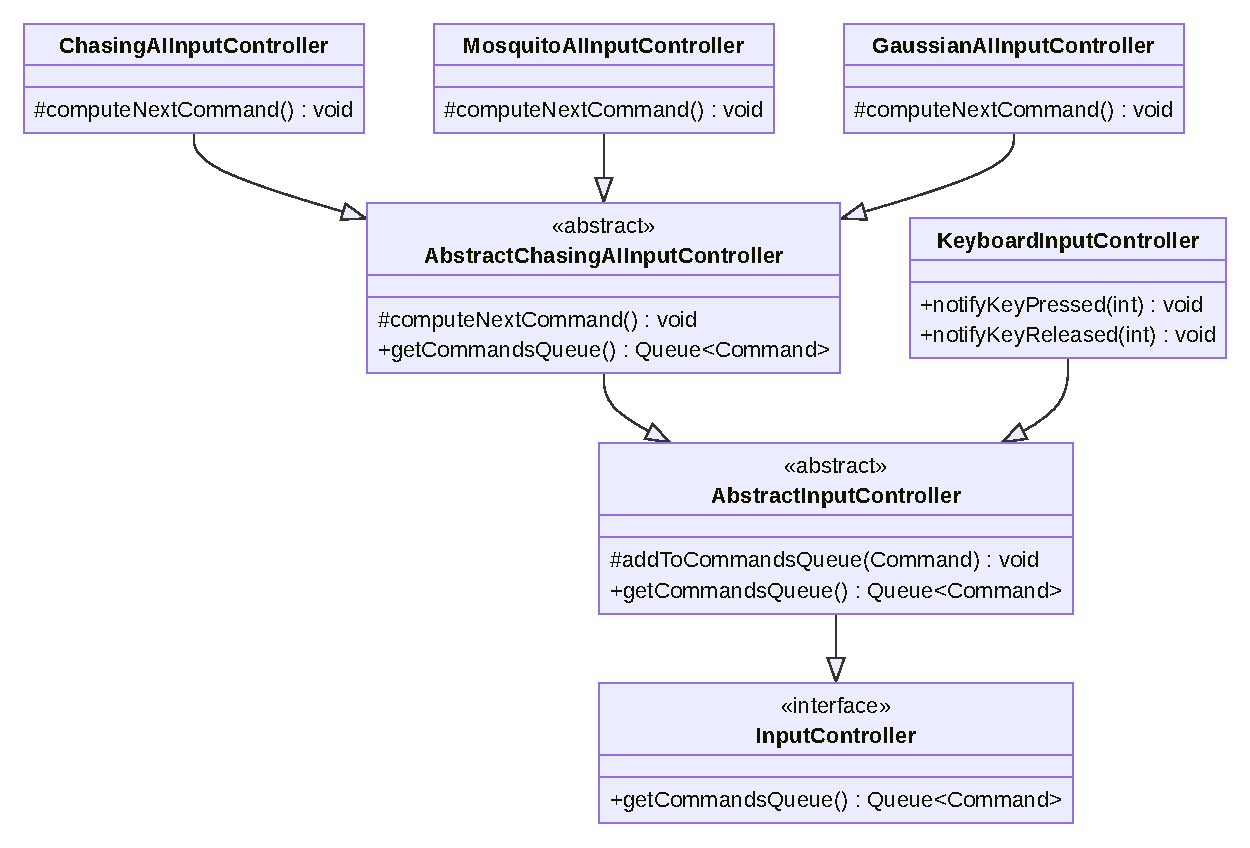
\includegraphics[scale=0.75]{img/InputControllerTemplateMethodUML}
\caption{Rappresentazione UML del pattern Template Method per il riuso di Input Controller}
\label{img:inputControllerTemplateMethod}
\end{figure}

\paragraph{Problema} Rendere riutilizzabili i comandi di gioco, separando la responsabilità di eseguirli dall’oggetto che li registra.

\paragraph{Soluzione} In \textit{AbstractInputController} viene data un’implementazione di default al metodo
\textit{getCommandsQueue()}, da questa classe astratta si possono costruire Input Controller 
come \textit{KeyboardInputController} che viene notificato ogni volta che un carattere da tastiera viene premuto
o rilasciato. Dato che un AI Input Controller non viene notificato da nessuna periferica, 
deve generare lui stesso i comandi da inserire nella \textit{commandsQueue}. 
Dato che diverse AI differiscono solamente per il metodo di generazione di comandi, è stato utilizzato il \textit{Template Method pattern}. 
\\
Nella classe \textit{AbstractChasingAIInputController} viene fatto l’override del metodo \textit{getCommandsQueue()} rendendolo il \textit{metodo di template} che, 
prima di ritornare la Commands Queue, chiama il metodo astratto \textit{computeNextCommand()}, 
il quale aggiunge in coda un comando generato seguendo l’algoritmo della data AI.

\subsubsection{Input Controller con molteplici stati}

\begin{figure}[H]
\centering{}
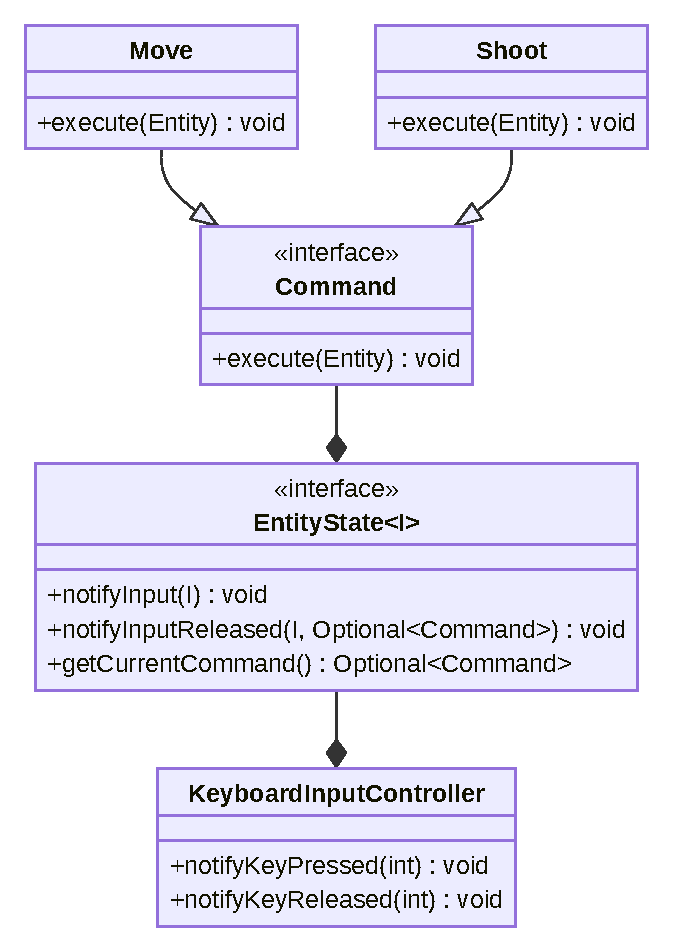
\includegraphics[scale=0.75]{img/EntityStateUML}
\caption{Rappresentazione UML del pattern State per la creazione di Input Controller con più FSM}
\label{img:inputControllerStatePattern}
\end{figure}

\paragraph{Problema} Rendere riutilizzabili i comandi di gioco, separando la responsabilità di eseguirli dall’oggetto che li registra.

\paragraph{Soluzione} Un player al momento presenta due \textit{macchine a stati finiti} (FSM): 
\textit{moveState} e \textit{shotState}. Ad ogni momento c'è un numero finito di stati in cui \textit{moveState} può stare: UP, DOWN, LEFT, RIGHT e STAY. 
Ad ognuno di questi stati corrisponde un comando (comportamento) diverso. \textit{moveState} può passare da uno stato ad un altro tramite regole dette \textit{transitions}, 
in questo caso le \textit{transitions} sono definite da un \textit{moveset} dove ad ogni input da tastiera corrisponde un comando. 
L'implementazione di questa FSM (e similmente anche per \textit{shotState}) è stata fatta utilizzando lo \textit{State pattern}, dove le implementazioni degli stati \textit{(Concrete States)} sono oggetti 
della classe \textit{Move} inizializzata con \textit{Directions} differenti, mentre il \textit{Context} è rappresentato da un implementazione di \textit{EntityState}. 
Grazie a questo pattern viene ridotta notevolmete la ripetizione di codice e semplificata l'aggiunta di ulteriori stati.
L'azione "sparare" è rappresentabile in quattro stati: UP, DOWN, LEFT, RIGHT; corrispondenti alla direzione del proitettile. Se "sparare" venisse trattato nella stessa FSM in cui viene gestito il movimento, per poter eseguire queste due azioni contemporaneamente, dovremmo duplicare il numero di stati.
Per risolvere questo problema vengono usate delle \textit{Concurrent State Machines}, ovvero due FSM che operano in maniera indipendente, in questo caso \textit{moveState} e \textit{shotState}.

\subsubsection{Gestione degli eventi di gioco}

\begin{figure}[H]
\centering{}
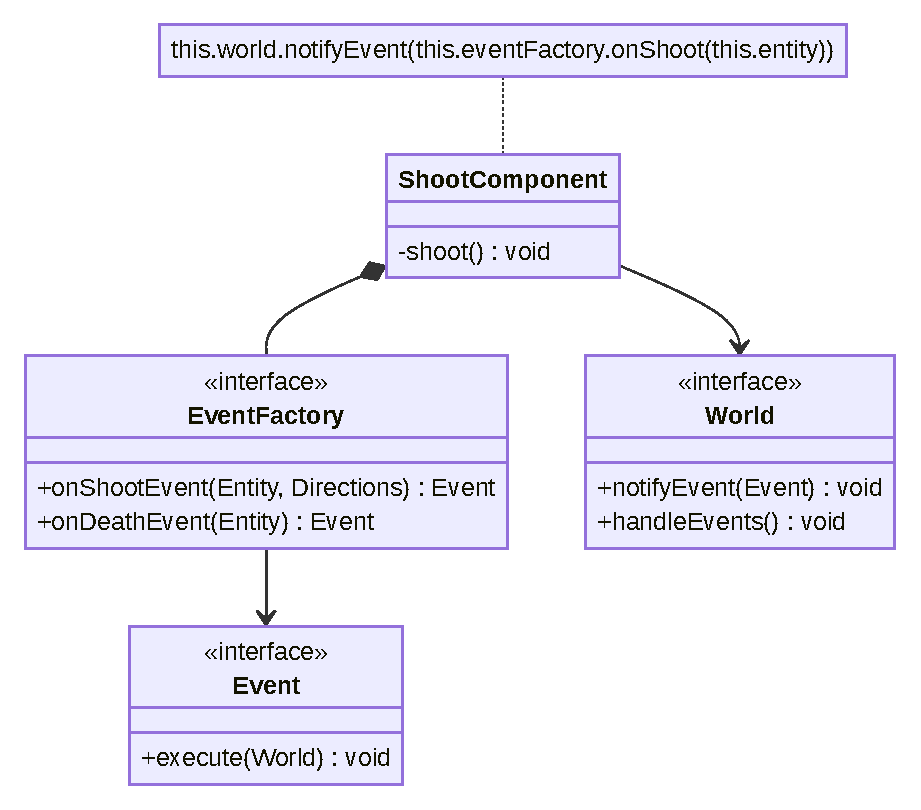
\includegraphics[scale=0.75]{img/EventsUML}
\caption{Rappresentazione UML della gestione degli eventi}
\label{img:eventsHandling}
\end{figure}

\paragraph{Problema} Dato che sono i Component a generare eventi, essi verrebbero generati quando viene chiamato il metodo \textit{update} di un component, quindi all’interno di un ciclo, incorrendo nel rischio di eccezioni \textit{“ConcurrentModificationException”}.

\paragraph{Soluzione} Per disaccoppiare l'evento generato da quando viene eseguito, utilizziamo il \textit{Pattern Event Queue}. 
Come descritto nel libro "Game Programming Patterns" di Robert Nystrom: \textit{"Una coda memorizza una serie di notifiche o richieste in ordine FIFO (First-In First-Out). 
Inviare una notifica aggiunge la richiesta alla coda e ritorna. Il "Request Processor" elabora quindi gli elementi nella coda in un secondo momento. 
Le richieste possono essere gestite direttamente o inoltrate ad altri oggetti. Questo disaccoppia il mittente dal destinatario sia staticamente che nel tempo"}
\footnote{\url{https://gameprogrammingpatterns.com/event-queue.html#the-pattern}}.
\\
Prendiamo come esempio l'evento \textit{onShoot}. La gestione degli eventi è analoga anche per \textit{onPowerUp} e \textit{onDeath}. Quando uno ShootComponent vuole generare un proiettile, chiama il metodo notifyEvent(Event) del \textit{Request Processor} World, 
passandogli un evento come parametro. Questo evento viene aggiunto alla coda della Event Queue. Gli eventi possono essere generati tramite una \textit{Factory}.
\\
Al prossimo update del Game, verrà chiamato il metodo handleEvents() del World, che eseguirà ogni comando presente nella coda, e poi la pulirà.
\subsection*{Fiumanò Luca Oskari}

\subsubsection{Gestione delle Wave}

\begin{figure}[H]
\centering{}
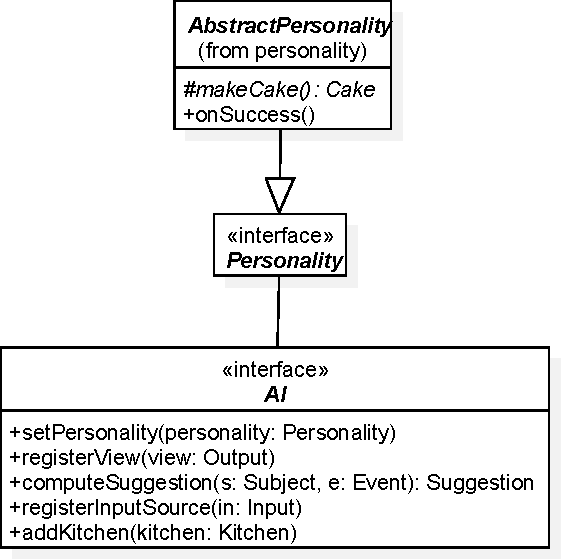
\includegraphics[width=\textwidth]{img/strategy}
\caption{Rappresentazione UML del pattern Factory per la gestione delle Wave}
\label{img:strategy}
\end{figure}

\paragraph{Problema} Esistono diversi tipi di Wave ognuna composta da nemici di vario tipo e numero.

\paragraph{Soluzione} Inizialmente per risolvere questo problema volevo utilizzare il \textit{Prototype} pattern creando una singola istanze per ogni tipo di nemico (prototipi) che sarebbero state clonate quando ritenute necessarie, inizialmente l’implementazione mi sembrava appropriata per risolvere il problema, ma non avevo preso in considerazione un problema fondamentale del pattern, infatti il metodo clone() che applicava il pattern non creava mai una nuova istanza ma passava solamente un riferimento del prototipo su cui era stato chiamato; questo causava diversi problemi, usando questo pattern i nemici avrebbero avuto tutti un riferimento agli stessi componenti questo causava ad esempio la condivisione di danno ricevuto tra tutti i nemici che avevano clonato lo stesso prototipo.
Ho capito quindi che sarebbe servito un pattern che creasse i diversi tipi di Wave formandole con istanze diverse di nemici; dopo un attenta ricerca la soluzione migliore mi è sembrata l’utilizzo di una \textit{Factory}. Così facendo mi sarei ritrovato nella condizione di poter creare un diverso tipo di wave con la sola chiamata di un metodo della \textit{Factory} senza incappare in errori di riferimenti comuni.

\subsubsection{Gestione delle Window indipendentemente dall'architettura grafica scelta}

\begin{figure}[H]
\centering{}
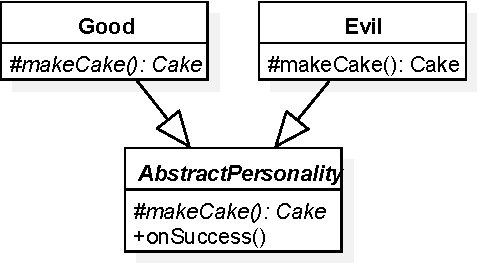
\includegraphics[width=\textwidth]{img/template}
\caption{Rappresentazione UML dell'applicazione del pattern Template Method alla Window}
\label{img:template}
\end{figure}

\paragraph{Problema} La gestione delle Window deve essere indipendente dall'architettura grafica scelta.

\paragraph{Soluzione} Per risolvere il problema ho deciso di utilizzare una classe astratta AbstractWindow che implementa il \textit{template method pattern} per definire come verranno create le scene. I template method sono \texttt{createGameScene()}, \texttt{createMenuScene()} e \texttt{createGameOverScene()} che utilizzano il metodo astratto \texttt{getSceneFactory()} che sarà implementato concretamente in una classe che estende AbstractWindow.

\subsubsection{Gestione delle diverse scene indipendentemente dall'architettura grafica scelta}

\begin{figure}[H]
\centering{}
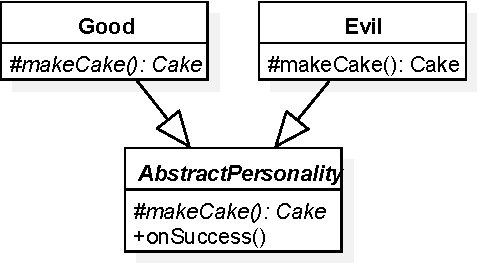
\includegraphics[width=\textwidth]{img/template}
\caption{Rappresentazione UML dell'applicazione del pattern FactoryMethod alla Scene}
\label{img:template}
\end{figure}

\paragraph{Problema} La gestione e creazione delle Scene deve essere indipendente dall'architettura grafica scelta.

\paragraph{Soluzione} Per venire a capo del problema ho deciso di utilizzare il \textit{pattern Factory} per delegare la creazione delle diverse scene in maniera indipendente dall'architettura grafica scelta; infatti se si volesse utilizzare una determinata architettura si dovrebbe creare una \textit{Factory} concreta per essa.

\subsubsection{Gestione di multipli PowerUp}

\begin{figure}[H]
\centering{}
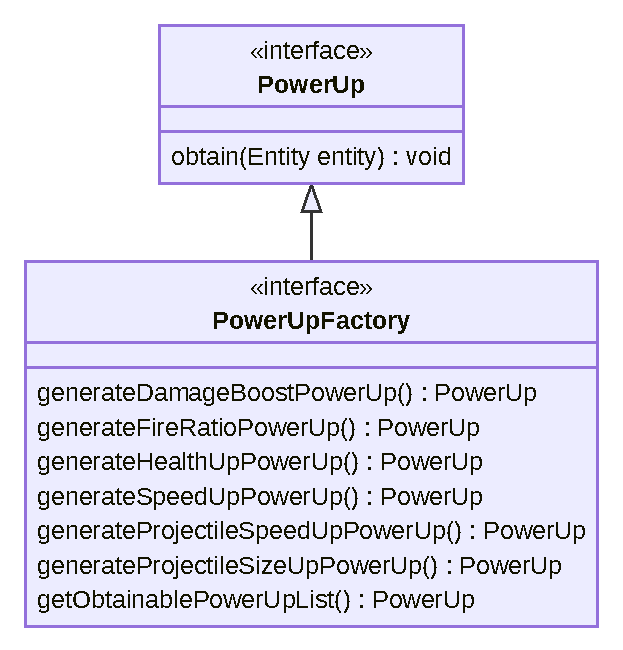
\includegraphics[width=\textwidth]{img/PowerUpUML}
\caption{Rappresentazione UML dell'applicazione del pattern Factory e Strategy ai PowerUp}
\label{img:observer}
\end{figure}

\paragraph{Problema} Il gioco deve implementare diversi tipi di PowerUp, ognuno che lavora su componenti diversi, che devono essere gestiti.

\paragraph{Soluzione} Dato che il nostro gioco doveva avere la possibilità di creare diversi tipi di PowerUp ognuno con comportamenti diversi ho deciso di utilizzare il \textit{Factory pattern} per sostituire la costruzione diretta dei PowerUp con delle appropriate chiamate alla \textit{Factory}. L'utilizzo del \textit{Factory method pattern} si è portato dietro un altro vantaggio la possibilità di aggiungere facilmente nuovi PowerUp.
Per risolvere il problema dei diversi comportamenti ho invece usato il pattern Strategy direttamente dentro la \textit{Factory} mediante il suo metodo privato \texttt{fromFunction()}.
\subsubsection{Riuso del codice delle personalità}

\begin{figure}[H]
\centering{}
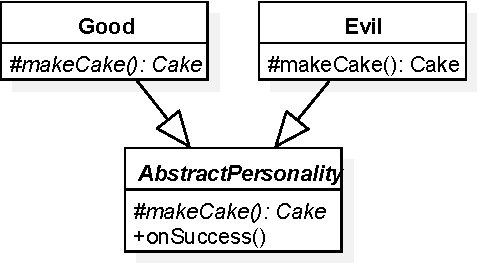
\includegraphics[width=\textwidth]{img/template}
\caption{Rappresentazione UML dell'applicazione del pattern Template Method alla gerarchia delle Personalità}
\label{img:template}
\end{figure}

\paragraph{Problema} In fase di sviluppo, sono state sviluppate due personalità, una buona ed una cattiva.
Quella buona restituisce sempre una torta vera, mentre quella cattiva restituisce sempre la
promessa di una torta che verrà in realtà disattesa.
Ci si è accorti che diverse personalità condividevano molto del comportamento,
portando a classi molto simili e a duplicazione.

\paragraph{Soluzione} Dato che le due personalità differiscono solo per il comportamento da effettuarsi in caso di percorso completato con successo,
è stato utilizzato il \textit{pattern template method} per massimizzare il riuso, come da \Cref{img:template}.
Il metodo template è \texttt{onSuccess()}, che chiama un metodo astratto e protetto
\texttt{makeCake()}.

\subsubsection{Gestione di output multipli}

\begin{figure}[H]
\centering{}
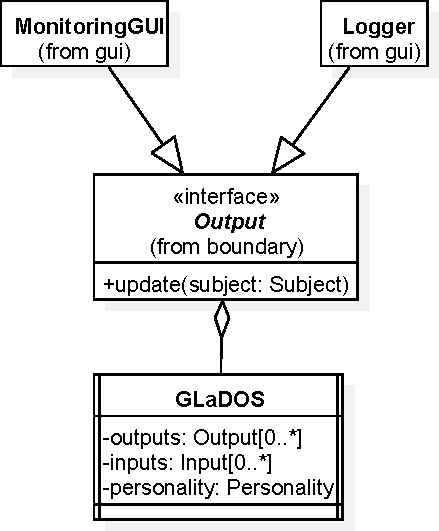
\includegraphics[width=.7\textwidth]{img/observer}
\caption{Il pattern Observer è usato per consentire a GLaDOS di informare tutti i sistemi di output in ascolto}
\label{img:observer}
\end{figure}

\paragraph{Problema} Il sistema deve supportare output multipli. In particolare, si richiede che vi sia un logger che stampa a terminale o su file,
e un'interfaccia grafica che mostri una rappresentazione grafica del sistema.

\paragraph{Soluzione} Dato che i due sistemi di reporting utilizzano le medesime informazioni, si è deciso di raggrupparli dietro l'interfaccia \texttt{Output}.
A questo punto, le due possibilità erano quelle di far sì che \texttt{GLaDOS} potesse pilotarle entrambe.
Invece di fare un sistema in cui questi output sono obbligatori e connessi, si è deciso di usare maggior flessibilità (anche in vista di future estensioni)
e di adottare una comunicazione uno-a-molti fra \texttt{GLaDOS} ed i sistemi di output.
La scelta è quindi ricaduta sul \textit{pattern Observer}: \texttt{GLaDOS} è observable, e le istanze di \texttt{Output} sono observer.
%
Il suo utilizzo è esemplificato in \Cref{img:observer}

\chapter{Sviluppo}
\section{Testing automatizzato}

Il testing automatizzato è un requisito di qualunque progetto software che si rispetti, e consente di verificare che non vi siano regressioni nelle funzionalità a fronte di aggiornamenti.
%
Per quanto riguarda questo progetto è considerato sufficiente un test minimale, a patto che sia completamente automatico.
%
Test che richiedono l'intervento da parte dell'utente sono considerati \textit{negativamente} nel computo del punteggio finale.

\subsection*{Elementi positivi}

\begin{itemize}
 \item Si descrivono molto brevemente i componenti che si è deciso di sottoporre a test automatizzato.
 \item Si utilizzano suite specifiche (e.g. JUnit) per il testing automatico.
\end{itemize}

\subsection*{Elementi negativi}
\begin{itemize}
 \item Non si realizza alcun test automatico.
 \item La non presenza di testing viene aggravata dall'adduzione di motivazioni non valide. Ad esempio, si scrive che l'interfaccia grafica non è testata automaticamente perché è \emph{impossibile} farlo\footnote{Testare in modo automatico le interfacce grafiche è possibile (si veda, come esempio, \url{https://github.com/TestFX/TestFX}), semplicemente nel corso non c'è modo e tempo di introdurvi questo livello di complessità. Il fatto che non vi sia stato insegnato come farlo non implica che sia impossibile!}.
 \item Si descrive un testing di tipo manuale in maniera prolissa.
 \item Si descrivono test effettuati manualmente che sarebbero potuti essere automatizzati, ad esempio scrivendo che si è usata l'applicazione manualmente.
 \item Si descrivono test non presenti nei sorgenti del progetto.
 \item I test, quando eseguiti, falliscono.
\end{itemize}

\section{Metodologia di lavoro}

Prima di cominciare con lo sviluppo abbiamo impostato l’architettura del gioco per avere delle solide fondamenta, iniziando con la definizione delle interfacce.
\\
La suddivisione iniziale del processo è stata fatta in maniera adeguata, consentendoci di lavorare parallelamente; riunendoci solo quando era necessario interlacciare le diverse implementazioni o per discutere su eventuali aggiunte.
\\
Abbiamo deciso di utilizzare il DVCS con il semplice approccio spiegato in classe, difatti dopo la creazione del repository ognuno di noi ne ha fatto un clone per lavorarci in autonomia condividendo le aggiunte mediante pull e push.

\subsection*{Nicolò D'Addabbo}
In autonomia mi sono occupato di:
\begin{itemize}
\item Input Component (in t2sgame.core.components)
\item Gestione degli input da periferica (package t2sgame.input)
\item AI (package t2sgame.input)
\item Comandi di gioco (package t2sgame.input)
\item Gestione degli eventi (Event ed EventFactory in t2sgame.logics e metodi notifyEvent e handleEvent in World)
\end{itemize}

\section{Note di sviluppo}

\subsection*{Nicolò D'Addabbo}
\subsubsection*{Utilizzo di Stream, lambda expression e method reference}
Usate molto spesso in vari punti del progetto:
\begin{itemize}
	\item Permalink: \url{https://github.com/nicolodaddabbo/OOP22-t2s-game/blob/d1453f9e5f56d2cdfec21561311304a309e99ed9/src/main/java/it/unibo/t2sgame/game/logics/impl/EventFactoryImpl.java#L37}
	\item Permalink: \url{https://github.com/nicolodaddabbo/OOP22-t2s-game/blob/d1453f9e5f56d2cdfec21561311304a309e99ed9/src/main/java/it/unibo/t2sgame/input/api/AbstractChasingAIInputController.java#L45-L48}
	\item Permalink: \url{https://github.com/nicolodaddabbo/OOP22-t2s-game/blob/d1453f9e5f56d2cdfec21561311304a309e99ed9/src/main/java/it/unibo/t2sgame/input/api/AbstractChasingAIInputController.java#L45-L48}
\end{itemize}
\subsubsection*{Classe con Generics}
\begin{itemize}
	\item Permalink: \url{https://github.com/nicolodaddabbo/OOP22-t2s-game/blob/d1453f9e5f56d2cdfec21561311304a309e99ed9/src/main/java/it/unibo/t2sgame/input/impl/EntityStateImpl.java#L14}
\end{itemize}

\chapter{Commenti finali}

\section{Autovalutazione e lavori futuri}
\subsection*{Nicolò D'Addabbo}
Sono soddisfatto del nostro progetto, che è stato un ottimo esercizio di lavoro di gruppo. Abbiamo collaborato in maniera efficace grazie a una buona fase di analisi, che è stata fondamentale per individuare quali problemi risolvere e come affrontarli. Questo progetto mi ha permesso di sviluppare abilità che possono essere applicate a progetti futuri, come la gestione del codice in gruppo ed una buona organizzazione del lavoro.
Ho lavorato alla parte Model e ho collaborato al Controller. Purtroppo non ho avuto la possibilità di approfondire JavaFX, che mi sarebbe interessato molto, poiché non ho avuto parti di View.

\appendix
\chapter{Guida utente}

Capitolo in cui si spiega come utilizzare il software. Nel caso in cui il suo uso sia del tutto
banale, tale capitolo può essere omesso.
%
A tal riguardo, si fa presente agli studenti che i docenti non hanno mai utilizzato il software
prima, per cui aspetti che sembrano del tutto banali a chi ha sviluppato l'applicazione possono non
esserlo per chi la usa per la prima volta.
%
Se, ad esempio, per cominciare una partita con un videogioco è necessario premere la barra
spaziatrice, o il tasto ``P'', è necessario che gli studenti lo segnalino.

\subsection*{Elementi positivi}

\begin{itemize}
 \item Si istruisce in modo semplice l'utente sull'uso dell'applicazione, eventualmente facendo uso di schermate e descrizioni.
\end{itemize}

\subsection*{Elementi negativi}
\begin{itemize}
 \item Si descrivono in modo eccessivamente minuzioso tutte le caratteristiche, anche minori, del software in oggetto.
 \item Manca una descrizione che consenta ad un utente qualunque di utilizzare almeno le funzionalità primarie dell'applicativo.
\end{itemize}

\bibliographystyle{alpha}
\bibliography{13-template}

\end{document}
